% Source-SHA256: cc2279a549f916466a8c2998206ec799ff902f69ae877d4291574b23b6ec9f3f
% !TeX program = lualatex
\documentclass[a4paper,11pt]{article}
\usepackage{fontspec}
\IfFontExistsTF{TeX Gyre Pagella}{\setmainfont{TeX Gyre Pagella}}{\setmainfont{P052}}
\IfFontExistsTF{TeX Gyre Heros}{\setsansfont{TeX Gyre Heros}}{\setsansfont{Nimbus Sans}}
\IfFontExistsTF{TeX Gyre Cursor}{\setmonofont{TeX Gyre Cursor}[Scale=0.88]}{\setmonofont{Nimbus Mono PS}[Scale=0.88]}
\usepackage{babel}
\babelprovide[import,main]{spanish}
\usepackage{microtype}
\usepackage[a4paper,margin=2.4cm,headheight=23pt,headsep=10pt,footskip=1.1cm]{geometry}
\raggedbottom
\setlength{\emergencystretch}{3em}
\hyphenpenalty=10000
\exhyphenpenalty=10000
\clubpenalty=10000
\widowpenalty=10000
\usepackage{xcolor}
\definecolor{navybg}{HTML}{0B1D2E}
\definecolor{navydeep}{HTML}{123049}
\definecolor{lightblue}{HTML}{8FD3FE}
\definecolor{amber}{HTML}{F5A623}
\definecolor{softgray}{HTML}{5B6570}
\usepackage{titlesec,needspace}
\setcounter{secnumdepth}{-1}
\setcounter{tocdepth}{2}
\titleformat{\section}{\sffamily\Large\bfseries\color{navydeep}\raggedright}{}{0pt}{}
\titleformat{\subsection}{\sffamily\large\bfseries\color{navydeep}\raggedright}{}{0pt}{}
\titlespacing*{\section}{0pt}{20pt}{9pt}
\titlespacing*{\subsection}{0pt}{14pt}{6pt}
\usepackage{fancyhdr}
\pagestyle{fancy}
\fancyhf{}
\fancyhead[L]{\small\sffamily\color{softgray}Drop Route}
\fancyhead[R]{\small\sffamily\color{softgray}Manual de instalación}
\fancyfoot[L]{\small\sffamily\color{softgray}Versión 1.1.0}
\fancyfoot[R]{\small\sffamily\color{softgray}\thepage}
\renewcommand{\headrulewidth}{0.4pt}
\usepackage{array,longtable,booktabs,calc}
\newcounter{none}
\renewcommand{\arraystretch}{1.15}
\usepackage{enumitem}
\setlist[itemize]{leftmargin=1.4em,itemsep=3pt,topsep=5pt}
\setlist[enumerate]{leftmargin=1.8em,itemsep=3pt,topsep=5pt}
\usepackage{fvextra,framed,seqsplit}
\fvset{fontsize=\small,breaklines=true,breakanywhere=true,frame=leftline,framerule=1.4pt,rulecolor=\color{lightblue},framesep=8pt}
\let\originaltexttt\texttt
\renewcommand{\texttt}[1]{\originaltexttt{\seqsplit{#1}}}
\providecommand{\tightlist}{\setlength{\itemsep}{2pt}\setlength{\parskip}{0pt}}
% Pandoc 3.2+ envuelve las imágenes en \pandocbounded; con versiones anteriores no existe y esta definición no cambia nada.
\providecommand{\pandocbounded}[1]{#1}
\usepackage{graphicx,xurl,wrapfig}
\usepackage[section]{placeins}
\usepackage{amssymb,newunicodechar}
\usepackage[colorlinks=true,linkcolor=navydeep,urlcolor=navydeep,pdftitle={Drop Route - Manual de instalación},pdfauthor={Jesús Quevedo Rodríguez}]{hyperref}
\usepackage{bookmark}
\newunicodechar{♭}{\texorpdfstring{\ensuremath{\flat}}{\unichar{9837}}}
\newunicodechar{♯}{\texorpdfstring{\ensuremath{\sharp}}{\unichar{9839}}}
\newunicodechar{✓}{\texorpdfstring{\ensuremath{\checkmark}}{\unichar{10003}}}
\newunicodechar{✗}{\texorpdfstring{\ensuremath{\times}}{\unichar{10007}}}
\newunicodechar{→}{\texorpdfstring{\ensuremath{\rightarrow}}{\unichar{8594}}}
\newunicodechar{←}{\texorpdfstring{\ensuremath{\leftarrow}}{\unichar{8592}}}
\setlength{\parindent}{0pt}
\setlength{\parskip}{6pt}
\renewcommand{\topfraction}{0.95}
\renewcommand{\bottomfraction}{0.95}
\renewcommand{\textfraction}{0.05}
\renewcommand{\floatpagefraction}{0.6}
\setcounter{topnumber}{3}
\setcounter{totalnumber}{4}
\begin{document}
\begin{titlepage}
\newgeometry{margin=0cm}
\thispagestyle{empty}
\pagecolor{navybg}
\color{white}
\vspace*{3cm}
\begin{center}
{\sffamily\bfseries\fontsize{16}{19}\selectfont\color{amber} DROP ROUTE\par}
\vspace{1.4cm}
{\sffamily\bfseries\fontsize{30}{38}\selectfont Manual de instalación\par}
\vspace{0.8cm}
{\sffamily\fontsize{14}{20}\selectfont\color{lightblue} Abrir, instalar y publicar la aplicación\par}
\vfill
{\sffamily\small Autor del proyecto: Jesús Quevedo Rodríguez\par}
{\sffamily\small Versión 1.1.0\par}
{\sffamily\small Repositorio: a01653/Drop\_Route\par}
\vspace{2cm}
\end{center}
\end{titlepage}
\nopagecolor
\restoregeometry
\setcounter{page}{2}
\tableofcontents
\newpage
Autor: Jesús Quevedo Rodríguez. Versión 1.1.0.

La aplicación se puede abrir en el navegador o instalar como PWA. La
dirección prevista para GitHub Pages es
\url{https://a01653.github.io/Drop_Route/}. Solo debe darse por activa
después de que el despliegue de \texttt{main} termine correctamente.

\section{1. Usar la aplicación
publicada}\label{1-usar-la-aplicaciuxf3n-publicada}

Abre la dirección HTTPS y espera a que aparezca el menú. La primera
carga completa permite que el service worker guarde los recursos
necesarios para el uso sin conexión.

En Android con Chrome, abre el menú del navegador y usa la opción de
instalación o creación de acceso directo que ofrezca la versión
instalada. En Chrome de escritorio puede aparecer \textbf{Instalar
página como aplicación}. En Safari de iPhone, usa \textbf{Compartir →
Añadir a pantalla de inicio}.

Los nombres exactos de los menús cambian según la versión del navegador.
La instalación PWA necesita HTTPS o \texttt{localhost}; una URL HTTP de
la red local no sirve para registrar el service worker.

\section{2. Probar desde el código}\label{2-probar-desde-el-cuxf3digo}

Requisitos para construir y servir la aplicación:

\begin{itemize}
\tightlist
\item
  Node.js 22.13 o posterior.
\item
  npm.
\item
  Git.
\end{itemize}

Clona el repositorio y carga las dependencias:

\begin{verbatim}
git clone https://github.com/a01653/Drop_Route.git Drop_Route
cd Drop_Route
npm ci --ignore-scripts
\end{verbatim}

Para desarrollo:

\begin{verbatim}
npm run dev
\end{verbatim}

Para probar el build que incluye la PWA:

\begin{verbatim}
npm run build
npm run preview
\end{verbatim}

\begin{figure}[!htbp]
\centering
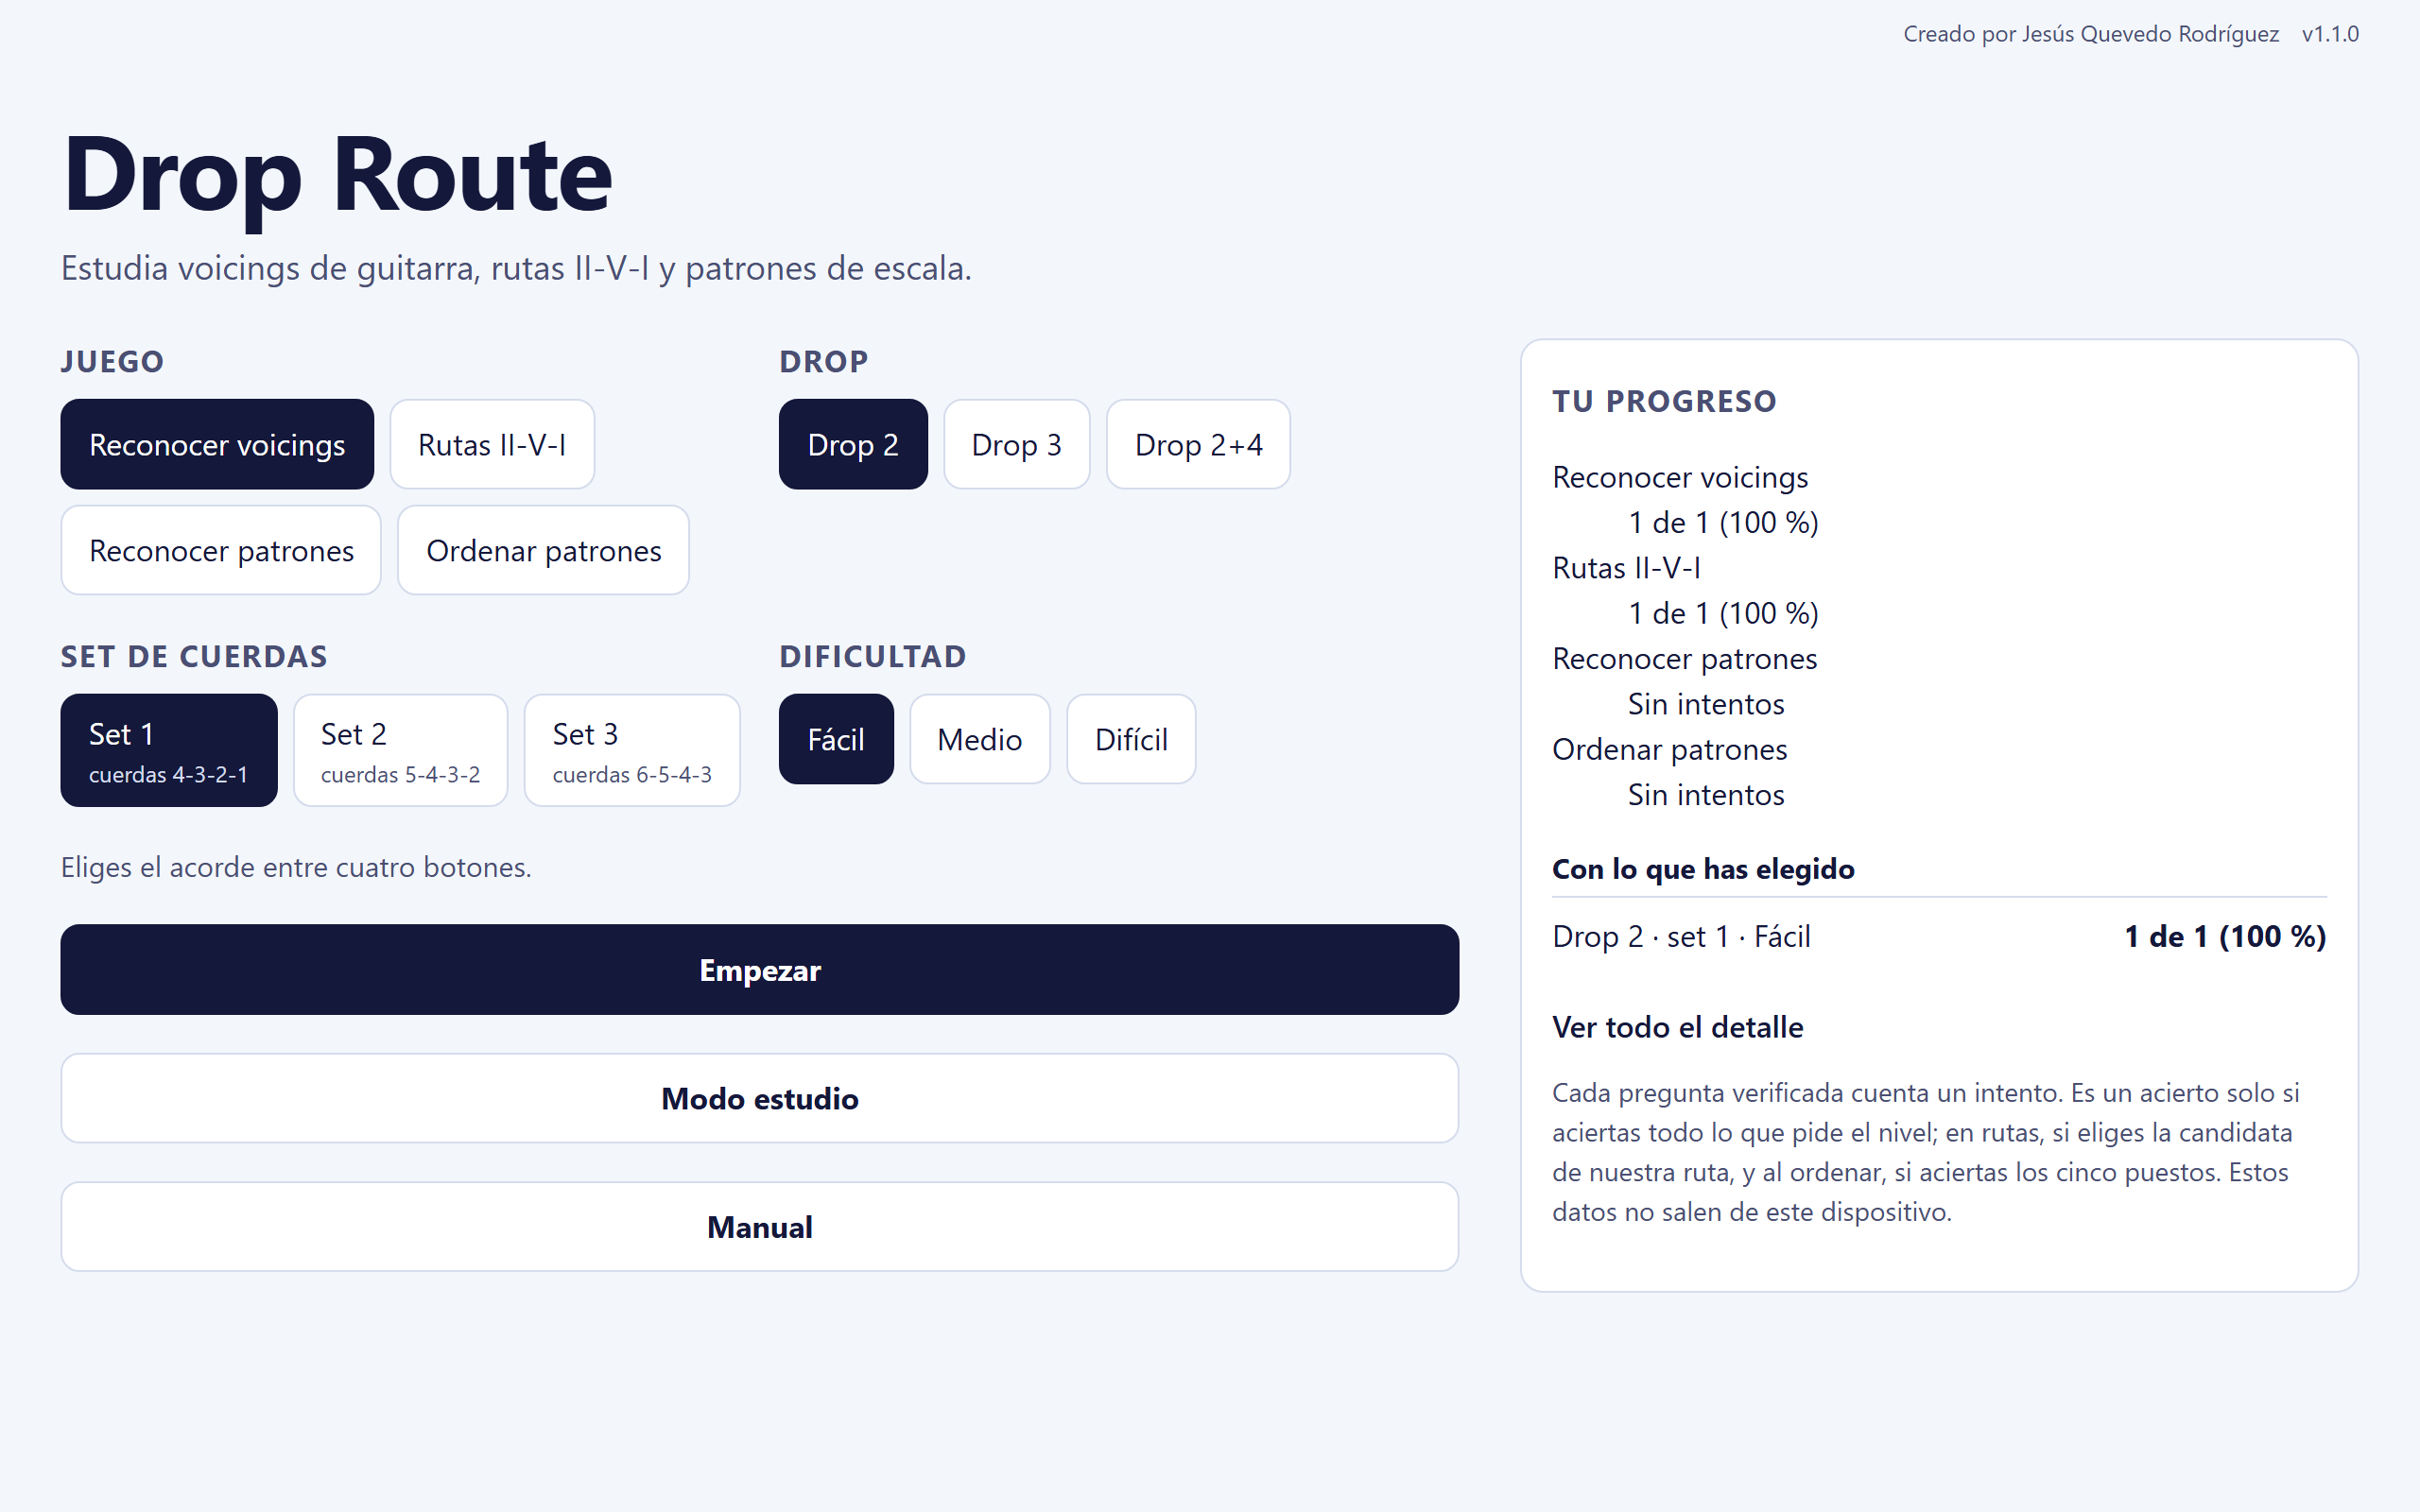
\includegraphics[width=0.82\linewidth,keepaspectratio]{../manuals/capturas/escritorio-menu-1280.png}\par\smallskip
{\footnotesize \emph{Figura 1. Vista de escritorio del build.}}
\end{figure}

\section{3. Publicar en la subruta de GitHub
Pages}\label{3-publicar-en-la-subruta-de-github-pages}

GitHub Pages sirve este repositorio bajo la ruta \texttt{/Drop\_Route/}.
El build debe conocer esa base:

\begin{verbatim}
DROP_ROUTE_BASE=/Drop_Route/ npm run build
\end{verbatim}

En PowerShell:

\begin{verbatim}
$env:DROP_ROUTE_BASE = '/Drop_Route/'
npm run build
\end{verbatim}

El resultado queda en \texttt{dist/}.

\section{4. GitHub Pages}\label{4-github-pages}

El workflow \texttt{.github/workflows/deploy-pages.yml} se ejecuta al
hacer push a \texttt{main} y también admite ejecución manual. Usa dos
trabajos: uno construye \texttt{dist/} con la base
\texttt{/Drop\_Route/}; el segundo publica el artefacto en GitHub Pages.

Si Pages aún no está activado en el repositorio, entra en
\textbf{Settings → Pages} y selecciona \textbf{GitHub Actions} como
origen. Después ejecuta de nuevo el workflow.

Cuando el despliegue termine en verde, comprueba
\url{https://a01653.github.io/Drop_Route/} con conexión y después una
recarga sin conexión.

\section{5. Pruebas opcionales}\label{5-pruebas-opcionales}

Para las pruebas E2E y las capturas de los manuales hace falta Chromium
de Playwright:

\begin{verbatim}
npx playwright install chromium
npm run test:e2e
npm run docs:captures
\end{verbatim}

La generación de los PDF de documentación usa Python 3.10 o posterior,
Pandoc y LuaLaTeX o XeLaTeX.
\end{document}
